\documentclass[11pt]{article}
\usepackage[utf8]{inputenc}
\usepackage{float}
\usepackage{amsmath}
\usepackage{tikz} % for Hasse diagram
\usepackage[hmargin=3cm,vmargin=6.0cm]{geometry}
%\topmargin=0cm
\topmargin=-2cm
\addtolength{\textheight}{6.5cm}
\addtolength{\textwidth}{2.0cm}
%\setlength{\leftmargin}{-5cm}
\setlength{\oddsidemargin}{0.0cm}
\setlength{\evensidemargin}{0.0cm}

\begin{document}
	
\section*{Student Information } 
%Write your full name and id number between the colon and newline
%Put one empty space character after colon and before newline
Full Name :  Ugur Duzel \\
Id Number :  2171569 \\

% Write your answers below the section tags
\section*{Answer 1}
Say, we have $n$ vertices that have the degree at least 4. \\
If we add all degrees of the vertices then this will be at least $4n$. Let $v$ be vertex and $V$ be set of the vertices in the graph. We can easily say, \\
$$4n \leq \sum_{v \in V}deg(v)$$
By Handshaking Theorem, we know that \\
$$2(Number\ of\ Edges)=\sum_{v \in V}deg(v)$$
So we can pass it into the previous inequality, \\
$$4n \leq 46$$
$$n \leq 11.5$$
This means number of vertices can be 11 at most. \\
Just a quick sanity check since these a small numbers, we can easily build this graph with 10 vertices having double loops and one vertex having one triple loop. Then we would have 11 vertices. \\

\section*{Answer 2}
Assuming that $G$ is simple graph with $n$ vertices. \\
Dirac's Theorem states that if each of the vertices has degree $d \geq \frac{n}{2}$\ where $n \geq 3$, then the graph $G$ contains Hamiltonian Circuit. Since this is still a circuit it must start and finish at the same vertex. Let's call this vertex $v_1$, the vertex after $v_1$ $v_2$ and the vertex just before the circuit is completed $v_k $\ (i.e. $v_2$ is the second vertex traveled in the circuit, $v_k$ is the vertex just before completing the circuit at $ v_1$ again). \\
Since $v_1$ is the first and the last vertex in the circuit, if we remove it and all the edges incident to it then we will not have a Hamiltonian Circuit but we will have Hamiltonian Path. It will start at $v_2$ and it will end at $v_k$. So this way, we always have a Hamiltonian Path if we remove the starting and the ending vertex (i.e. $v_1$). We would have one less vertex so this is possible if each of the vertices of the simple graph $G$, has degree $d \geq \frac{n-1}{2}$ and $n \geq 3$.
\vspace{2cm}
\section*{Answer 3}
A bipartite graph $G$ is a graph whose set of vertices $V$ can be partitioned into two nonempty subsets $V_1$ and $V_2$ such that every edge in $G$ connects $V_1$ and $V_2$. Therefore, the first neighbors of vertices in $V_1$ are contained in $V_2$ and vice versa. Let's say $1,\ 2,\ ...,\ m$ belong to the subset $V_1$ and vertices $p+1,\ p+2,\ ...,\ p+n$ belong to $V_2$ then the corresponding adjacency matrix is going to be,
\[
A=
  \begin{bmatrix}
    0 & B \\
    B^T & 0
  \end{bmatrix}
\] 
where $B$ is a sub-matrix with dimensions $m$ x $n$, $B^T$ is its transpose and $0$ are the zero matrices of the size determined by the sub-matrices. Then we can say,  \\
\[
A^2=
  \begin{bmatrix}
    B B^T & 0 \\
   0 & B^T B
  \end{bmatrix}
\] \\
\[
A^3=
  \begin{bmatrix}
    0 & B B^T B \\
    B^T B B^T & 0
  \end{bmatrix}
\] \\
Considering this pattern we can easily determine that $A^k$ always has 0 on its diagonal when  k is odd. Since 37 is an odd number the final matrix will have the form, \\\
\[
A^{37}=
  \begin{bmatrix}
    0 & B B^T B B^T\ ...\ B^T B \\
    B^T B B^T B\ ...\ B B^T & 0
  \end{bmatrix}
\] \\
So as we can see the diagonal is all $0$.


\section*{Answer 4}

\vspace{1cm}
\begin{itemize}
	\item[\textbf{a.}] 
------------------------------------------------------------------------------------------------------------------------------------
		\begin{figure}[H]	
		\centering
		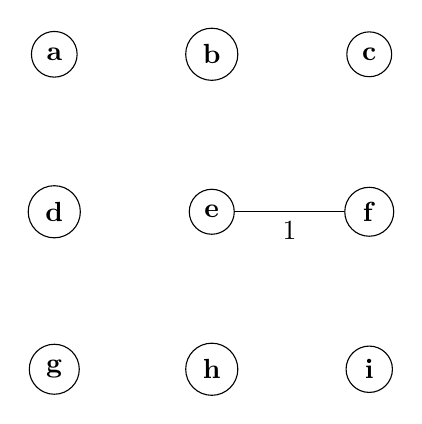
\begin{tikzpicture}

		\node[shape=circle,draw=black] (a) at (0, 4)     {\textbf{a}};
		\node[shape=circle,draw=black] (b) at (2, 4)     {\textbf{b}};
		\node[shape=circle,draw=black] (c) at (4, 4)     {\textbf{c}};
		\node[shape=circle,draw=black] (d) at (0, 2)     {\textbf{d}};
		\node[shape=circle,draw=black] (e) at (2, 2)     {\textbf{e}};
		\node[shape=circle,draw=black] (f) at (4, 2)     {\textbf{f}};
		\node[shape=circle,draw=black] (g) at (0, 0)     {\textbf{g}};
		\node[shape=circle,draw=black] (h) at (2, 0)     {\textbf{h}};
		\node[shape=circle,draw=black] (i) at (4, 0)     {\textbf{i}};
		\path[-] (e) edge  node[below] {1} (f);
	
		\end{tikzpicture} 
	\end{figure}	
------------------------------------------------------------------------------------------------------------------------------------
\begin{figure}[H]	
	\centering
	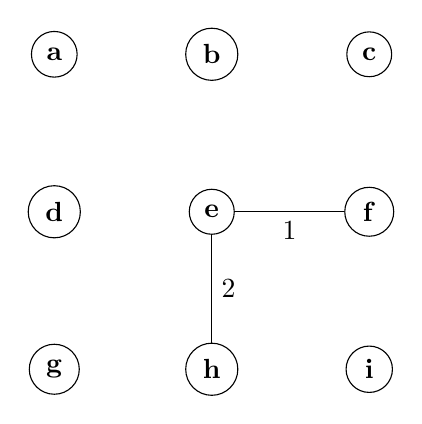
\begin{tikzpicture}
	
	\node[shape=circle,draw=black] (a) at (0, 4)     {\textbf{a}};
	\node[shape=circle,draw=black] (b) at (2, 4)     {\textbf{b}};
	\node[shape=circle,draw=black] (c) at (4, 4)     {\textbf{c}};
	\node[shape=circle,draw=black] (d) at (0, 2)     {\textbf{d}};
	\node[shape=circle,draw=black] (e) at (2, 2)     {\textbf{e}};
	\node[shape=circle,draw=black] (f) at (4, 2)     {\textbf{f}};
	\node[shape=circle,draw=black] (g) at (0, 0)     {\textbf{g}};
	\node[shape=circle,draw=black] (h) at (2, 0)     {\textbf{h}};
	\node[shape=circle,draw=black] (i) at (4, 0)     {\textbf{i}};
	\path[-] (e) edge  node[below] {1} (f);
	\path[-] (e) edge  node[right] {2} (h);
	
	\end{tikzpicture} 
\end{figure}	
------------------------------------------------------------------------------------------------------------------------------------
\begin{figure}[H]	
	\centering
	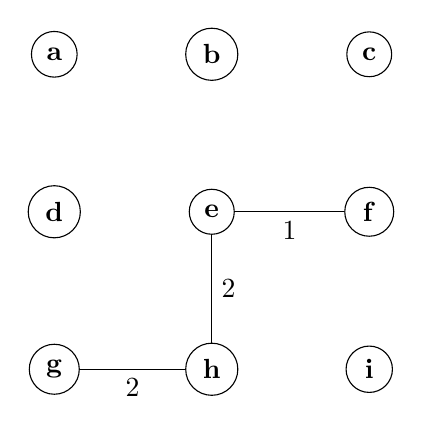
\begin{tikzpicture}
	
	\node[shape=circle,draw=black] (a) at (0, 4)     {\textbf{a}};
	\node[shape=circle,draw=black] (b) at (2, 4)     {\textbf{b}};
	\node[shape=circle,draw=black] (c) at (4, 4)     {\textbf{c}};
	\node[shape=circle,draw=black] (d) at (0, 2)     {\textbf{d}};
	\node[shape=circle,draw=black] (e) at (2, 2)     {\textbf{e}};
	\node[shape=circle,draw=black] (f) at (4, 2)     {\textbf{f}};
	\node[shape=circle,draw=black] (g) at (0, 0)     {\textbf{g}};
	\node[shape=circle,draw=black] (h) at (2, 0)     {\textbf{h}};
	\node[shape=circle,draw=black] (i) at (4, 0)     {\textbf{i}};
	\path[-] (e) edge  node[below] {1} (f);
	\path[-] (e) edge  node[right] {2} (h);
	\path[-] (g) edge  node[below] {2} (h);
	
	\end{tikzpicture} 
\end{figure}
------------------------------------------------------------------------------------------------------------------------------------
\begin{figure}[H]	
	\centering
	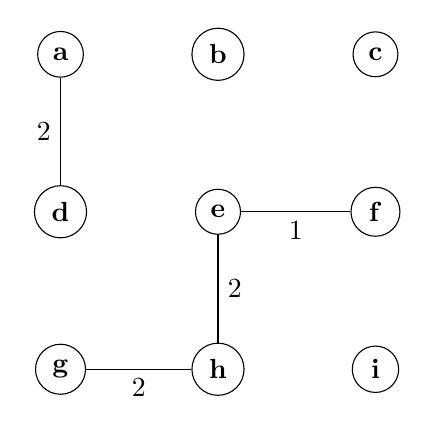
\begin{tikzpicture}
	
	\node[shape=circle,draw=black] (a) at (0, 4)     {\textbf{a}};
	\node[shape=circle,draw=black] (b) at (2, 4)     {\textbf{b}};
	\node[shape=circle,draw=black] (c) at (4, 4)     {\textbf{c}};
	\node[shape=circle,draw=black] (d) at (0, 2)     {\textbf{d}};
	\node[shape=circle,draw=black] (e) at (2, 2)     {\textbf{e}};
	\node[shape=circle,draw=black] (f) at (4, 2)     {\textbf{f}};
	\node[shape=circle,draw=black] (g) at (0, 0)     {\textbf{g}};
	\node[shape=circle,draw=black] (h) at (2, 0)     {\textbf{h}};
	\node[shape=circle,draw=black] (i) at (4, 0)     {\textbf{i}};
	\path[-] (e) edge  node[below] {1} (f);
	\path[-] (e) edge  node[right] {2} (h);
	\path[-] (g) edge  node[below] {2} (h);
	\path[-] (a) edge  node[left]  {2} (d);
	
	\end{tikzpicture} 
\end{figure}
------------------------------------------------------------------------------------------------------------------------------------
\begin{figure}[H]	
	\centering
	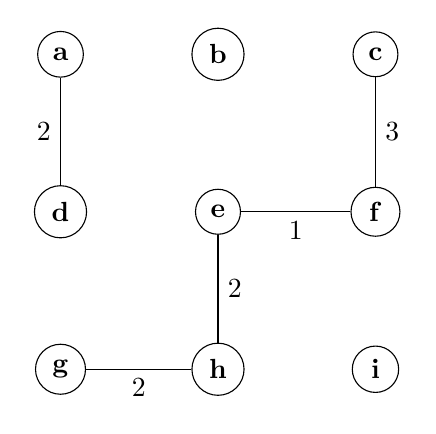
\begin{tikzpicture}
	
	\node[shape=circle,draw=black] (a) at (0, 4)     {\textbf{a}};
	\node[shape=circle,draw=black] (b) at (2, 4)     {\textbf{b}};
	\node[shape=circle,draw=black] (c) at (4, 4)     {\textbf{c}};
	\node[shape=circle,draw=black] (d) at (0, 2)     {\textbf{d}};
	\node[shape=circle,draw=black] (e) at (2, 2)     {\textbf{e}};
	\node[shape=circle,draw=black] (f) at (4, 2)     {\textbf{f}};
	\node[shape=circle,draw=black] (g) at (0, 0)     {\textbf{g}};
	\node[shape=circle,draw=black] (h) at (2, 0)     {\textbf{h}};
	\node[shape=circle,draw=black] (i) at (4, 0)     {\textbf{i}};
	\path[-] (e) edge  node[below] {1} (f);
	\path[-] (e) edge  node[right] {2} (h);
	\path[-] (g) edge  node[below] {2} (h);
	\path[-] (a) edge  node[left]  {2} (d);
	\path[-] (c) edge  node[right] {3} (f);
	
	\end{tikzpicture} 
\end{figure}	
------------------------------------------------------------------------------------------------------------------------------------
\begin{figure}[H]	
	\centering
	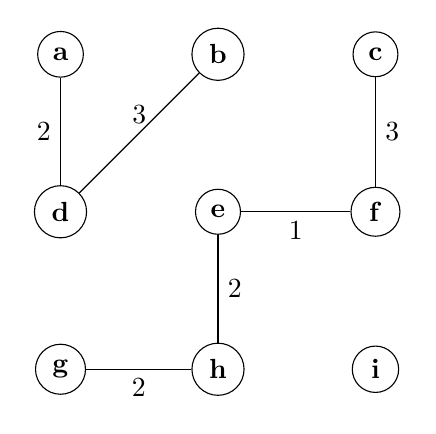
\begin{tikzpicture}
	
	\node[shape=circle,draw=black] (a) at (0, 4)     {\textbf{a}};
	\node[shape=circle,draw=black] (b) at (2, 4)     {\textbf{b}};
	\node[shape=circle,draw=black] (c) at (4, 4)     {\textbf{c}};
	\node[shape=circle,draw=black] (d) at (0, 2)     {\textbf{d}};
	\node[shape=circle,draw=black] (e) at (2, 2)     {\textbf{e}};
	\node[shape=circle,draw=black] (f) at (4, 2)     {\textbf{f}};
	\node[shape=circle,draw=black] (g) at (0, 0)     {\textbf{g}};
	\node[shape=circle,draw=black] (h) at (2, 0)     {\textbf{h}};
	\node[shape=circle,draw=black] (i) at (4, 0)     {\textbf{i}};
	\path[-] (e) edge  node[below] {1} (f);
	\path[-] (e) edge  node[right] {2} (h);
	\path[-] (g) edge  node[below] {2} (h);
	\path[-] (a) edge  node[left]  {2} (d);
	\path[-] (c) edge  node[right] {3} (f);
	\path[-] (b) edge  node[above] {3} (d);
	
	\end{tikzpicture} 
\end{figure}
------------------------------------------------------------------------------------------------------------------------------------
\begin{figure}[H]	
	\centering
	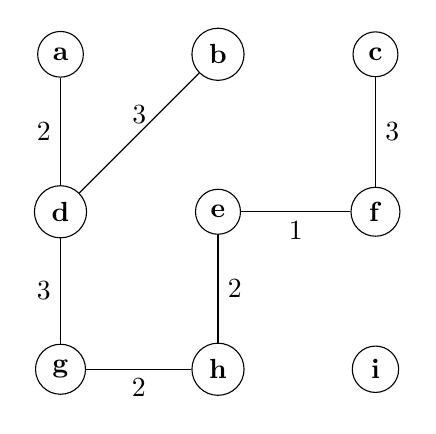
\begin{tikzpicture}
	
	\node[shape=circle,draw=black] (a) at (0, 4)     {\textbf{a}};
	\node[shape=circle,draw=black] (b) at (2, 4)     {\textbf{b}};
	\node[shape=circle,draw=black] (c) at (4, 4)     {\textbf{c}};
	\node[shape=circle,draw=black] (d) at (0, 2)     {\textbf{d}};
	\node[shape=circle,draw=black] (e) at (2, 2)     {\textbf{e}};
	\node[shape=circle,draw=black] (f) at (4, 2)     {\textbf{f}};
	\node[shape=circle,draw=black] (g) at (0, 0)     {\textbf{g}};
	\node[shape=circle,draw=black] (h) at (2, 0)     {\textbf{h}};
	\node[shape=circle,draw=black] (i) at (4, 0)     {\textbf{i}};
	\path[-] (e) edge  node[below] {1} (f);
	\path[-] (e) edge  node[right] {2} (h);
	\path[-] (g) edge  node[below] {2} (h);
	\path[-] (a) edge  node[left]  {2} (d);
	\path[-] (c) edge  node[right] {3} (f);
	\path[-] (b) edge  node[above] {3} (d);
	\path[-] (d) edge  node[left]  {3} (g);
	
	\end{tikzpicture} 
\end{figure}
------------------------------------------------------------------------------------------------------------------------------------
\begin{figure}[H]	
	\centering
	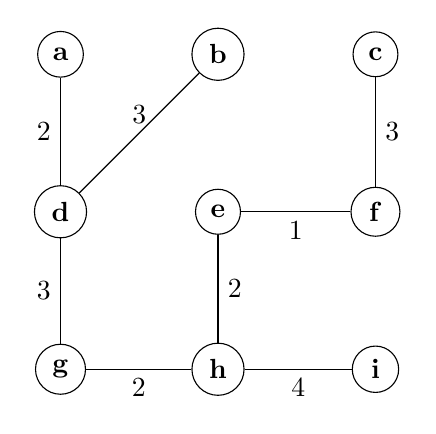
\begin{tikzpicture}
	
	\node[shape=circle,draw=black] (a) at (0, 4)     {\textbf{a}};
	\node[shape=circle,draw=black] (b) at (2, 4)     {\textbf{b}};
	\node[shape=circle,draw=black] (c) at (4, 4)     {\textbf{c}};
	\node[shape=circle,draw=black] (d) at (0, 2)     {\textbf{d}};
	\node[shape=circle,draw=black] (e) at (2, 2)     {\textbf{e}};
	\node[shape=circle,draw=black] (f) at (4, 2)     {\textbf{f}};
	\node[shape=circle,draw=black] (g) at (0, 0)     {\textbf{g}};
	\node[shape=circle,draw=black] (h) at (2, 0)     {\textbf{h}};
	\node[shape=circle,draw=black] (i) at (4, 0)     {\textbf{i}};
	\path[-] (e) edge  node[below] {1} (f);
	\path[-] (e) edge  node[right] {2} (h);
	\path[-] (g) edge  node[below] {2} (h);
	\path[-] (a) edge  node[left]  {2} (d);
	\path[-] (c) edge  node[right] {3} (f);
	\path[-] (b) edge  node[above] {3} (d);
	\path[-] (d) edge  node[left]  {3} (g);
	\path[-] (h) edge  node[below] {4} (i);
	
	\end{tikzpicture} 
\end{figure}	

	\item[\textbf{b.}] 
------------------------------------------------------------------------------------------------------------------------------------
\begin{figure}[H]	
	\centering
	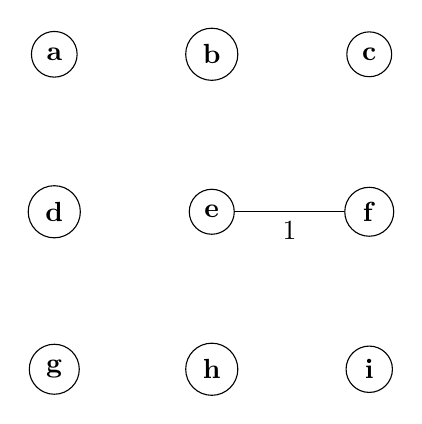
\begin{tikzpicture}	
	
	\node[shape=circle,draw=black] (a) at (0, 4)     {\textbf{a}};
	\node[shape=circle,draw=black] (b) at (2, 4)     {\textbf{b}};
	\node[shape=circle,draw=black] (c) at (4, 4)     {\textbf{c}};
	\node[shape=circle,draw=black] (d) at (0, 2)     {\textbf{d}};
	\node[shape=circle,draw=black] (e) at (2, 2)     {\textbf{e}};
	\node[shape=circle,draw=black] (f) at (4, 2)     {\textbf{f}};
	\node[shape=circle,draw=black] (g) at (0, 0)     {\textbf{g}};
	\node[shape=circle,draw=black] (h) at (2, 0)     {\textbf{h}};
	\node[shape=circle,draw=black] (i) at (4, 0)     {\textbf{i}};
	\path[-] (e) edge  node[below] {1} (f);

	
	\end{tikzpicture} 
\end{figure}
------------------------------------------------------------------------------------------------------------------------------------
\begin{figure}[H]	
	\centering
	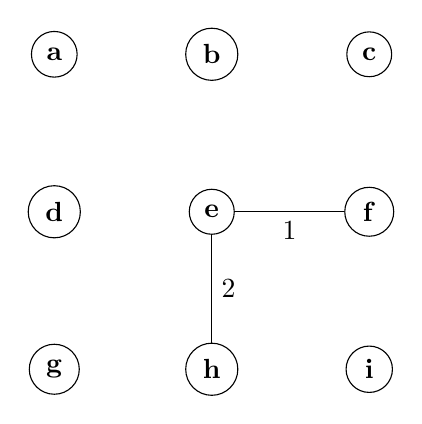
\begin{tikzpicture}	
	
	\node[shape=circle,draw=black] (a) at (0, 4)     {\textbf{a}};
	\node[shape=circle,draw=black] (b) at (2, 4)     {\textbf{b}};
	\node[shape=circle,draw=black] (c) at (4, 4)     {\textbf{c}};
	\node[shape=circle,draw=black] (d) at (0, 2)     {\textbf{d}};
	\node[shape=circle,draw=black] (e) at (2, 2)     {\textbf{e}};
	\node[shape=circle,draw=black] (f) at (4, 2)     {\textbf{f}};
	\node[shape=circle,draw=black] (g) at (0, 0)     {\textbf{g}};
	\node[shape=circle,draw=black] (h) at (2, 0)     {\textbf{h}};
	\node[shape=circle,draw=black] (i) at (4, 0)     {\textbf{i}};
	\path[-] (e) edge  node[below] {1} (f);
	\path[-] (e) edge  node[right] {2} (h);
	
	\end{tikzpicture} 
\end{figure}
------------------------------------------------------------------------------------------------------------------------------------
\begin{figure}[H]	
	\centering
	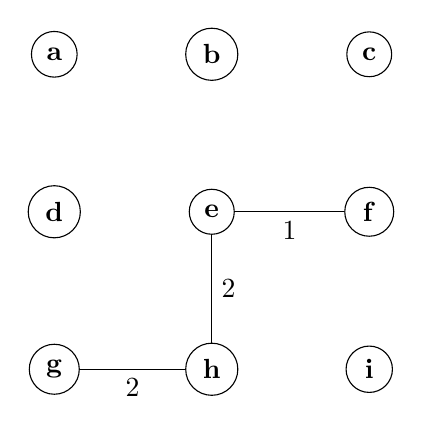
\begin{tikzpicture}	
	
	\node[shape=circle,draw=black] (a) at (0, 4)     {\textbf{a}};
	\node[shape=circle,draw=black] (b) at (2, 4)     {\textbf{b}};
	\node[shape=circle,draw=black] (c) at (4, 4)     {\textbf{c}};
	\node[shape=circle,draw=black] (d) at (0, 2)     {\textbf{d}};
	\node[shape=circle,draw=black] (e) at (2, 2)     {\textbf{e}};
	\node[shape=circle,draw=black] (f) at (4, 2)     {\textbf{f}};
	\node[shape=circle,draw=black] (g) at (0, 0)     {\textbf{g}};
	\node[shape=circle,draw=black] (h) at (2, 0)     {\textbf{h}};
	\node[shape=circle,draw=black] (i) at (4, 0)     {\textbf{i}};
	\path[-] (e) edge  node[below] {1} (f);
	\path[-] (e) edge  node[right] {2} (h);
	\path[-] (g) edge  node[below] {2} (h);
	
	\end{tikzpicture} 
\end{figure}
------------------------------------------------------------------------------------------------------------------------------------
\begin{figure}[H]	
	\centering
	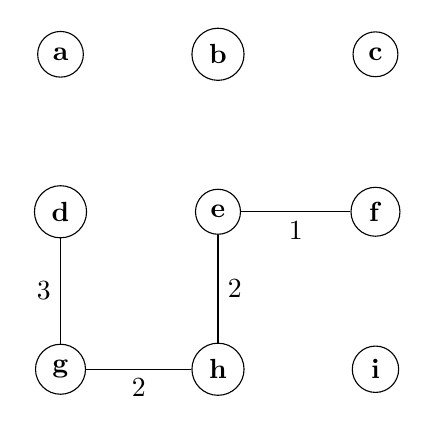
\begin{tikzpicture}	
	
	\node[shape=circle,draw=black] (a) at (0, 4)     {\textbf{a}};
	\node[shape=circle,draw=black] (b) at (2, 4)     {\textbf{b}};
	\node[shape=circle,draw=black] (c) at (4, 4)     {\textbf{c}};
	\node[shape=circle,draw=black] (d) at (0, 2)     {\textbf{d}};
	\node[shape=circle,draw=black] (e) at (2, 2)     {\textbf{e}};
	\node[shape=circle,draw=black] (f) at (4, 2)     {\textbf{f}};
	\node[shape=circle,draw=black] (g) at (0, 0)     {\textbf{g}};
	\node[shape=circle,draw=black] (h) at (2, 0)     {\textbf{h}};
	\node[shape=circle,draw=black] (i) at (4, 0)     {\textbf{i}};
	\path[-] (e) edge  node[below] {1} (f);
	\path[-] (e) edge  node[right] {2} (h);
	\path[-] (g) edge  node[below] {2} (h);
	\path[-] (d) edge  node[left]  {3} (g);
	
	\end{tikzpicture} 
\end{figure}
------------------------------------------------------------------------------------------------------------------------------------
\begin{figure}[H]	
	\centering
	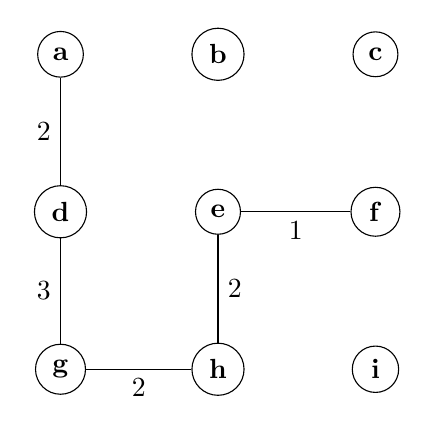
\begin{tikzpicture}	
	
	\node[shape=circle,draw=black] (a) at (0, 4)     {\textbf{a}};
	\node[shape=circle,draw=black] (b) at (2, 4)     {\textbf{b}};
	\node[shape=circle,draw=black] (c) at (4, 4)     {\textbf{c}};
	\node[shape=circle,draw=black] (d) at (0, 2)     {\textbf{d}};
	\node[shape=circle,draw=black] (e) at (2, 2)     {\textbf{e}};
	\node[shape=circle,draw=black] (f) at (4, 2)     {\textbf{f}};
	\node[shape=circle,draw=black] (g) at (0, 0)     {\textbf{g}};
	\node[shape=circle,draw=black] (h) at (2, 0)     {\textbf{h}};
	\node[shape=circle,draw=black] (i) at (4, 0)     {\textbf{i}};
	\path[-] (e) edge  node[below] {1} (f);
	\path[-] (e) edge  node[right] {2} (h);
	\path[-] (g) edge  node[below] {2} (h);
	\path[-] (d) edge  node[left]  {3} (g);
	\path[-] (a) edge  node[left]  {2} (d);
	
	\end{tikzpicture} 
\end{figure}
------------------------------------------------------------------------------------------------------------------------------------
\begin{figure}[H]	
	\centering
	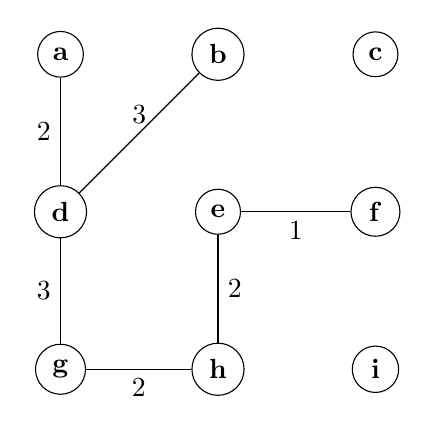
\begin{tikzpicture}	
	
	\node[shape=circle,draw=black] (a) at (0, 4)     {\textbf{a}};
	\node[shape=circle,draw=black] (b) at (2, 4)     {\textbf{b}};
	\node[shape=circle,draw=black] (c) at (4, 4)     {\textbf{c}};
	\node[shape=circle,draw=black] (d) at (0, 2)     {\textbf{d}};
	\node[shape=circle,draw=black] (e) at (2, 2)     {\textbf{e}};
	\node[shape=circle,draw=black] (f) at (4, 2)     {\textbf{f}};
	\node[shape=circle,draw=black] (g) at (0, 0)     {\textbf{g}};
	\node[shape=circle,draw=black] (h) at (2, 0)     {\textbf{h}};
	\node[shape=circle,draw=black] (i) at (4, 0)     {\textbf{i}};
	\path[-] (e) edge  node[below] {1} (f);
	\path[-] (e) edge  node[right] {2} (h);
	\path[-] (g) edge  node[below] {2} (h);
	\path[-] (d) edge  node[left]  {3} (g);
	\path[-] (a) edge  node[left]  {2} (d);
	\path[-] (b) edge  node[above] {3} (d);
	
	\end{tikzpicture} 
\end{figure}
------------------------------------------------------------------------------------------------------------------------------------
\begin{figure}[H]	
	\centering
	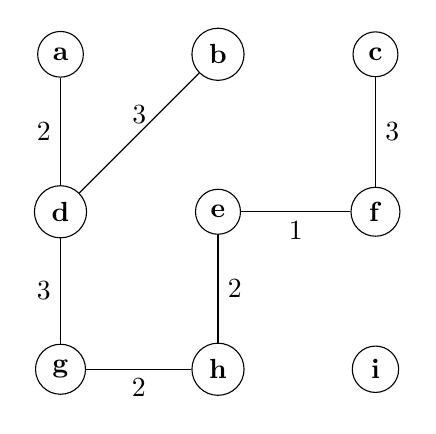
\begin{tikzpicture}	
	
	\node[shape=circle,draw=black] (a) at (0, 4)     {\textbf{a}};
	\node[shape=circle,draw=black] (b) at (2, 4)     {\textbf{b}};
	\node[shape=circle,draw=black] (c) at (4, 4)     {\textbf{c}};
	\node[shape=circle,draw=black] (d) at (0, 2)     {\textbf{d}};
	\node[shape=circle,draw=black] (e) at (2, 2)     {\textbf{e}};
	\node[shape=circle,draw=black] (f) at (4, 2)     {\textbf{f}};
	\node[shape=circle,draw=black] (g) at (0, 0)     {\textbf{g}};
	\node[shape=circle,draw=black] (h) at (2, 0)     {\textbf{h}};
	\node[shape=circle,draw=black] (i) at (4, 0)     {\textbf{i}};
	\path[-] (e) edge  node[below] {1} (f);
	\path[-] (e) edge  node[right] {2} (h);
	\path[-] (g) edge  node[below] {2} (h);
	\path[-] (d) edge  node[left]  {3} (g);
	\path[-] (a) edge  node[left]  {2} (d);
	\path[-] (b) edge  node[above] {3} (d);
	\path[-] (c) edge  node[right] {3} (f);
	
	\end{tikzpicture} 
\end{figure}
------------------------------------------------------------------------------------------------------------------------------------
\begin{figure}[H]	
	\centering
	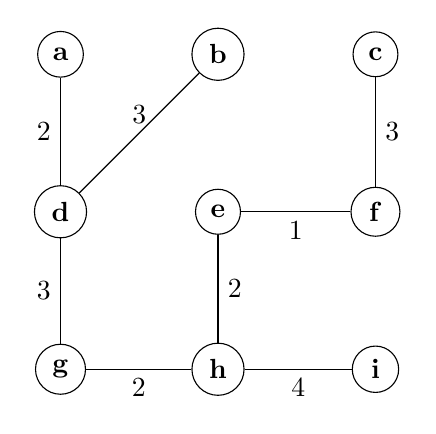
\begin{tikzpicture}	
	
	\node[shape=circle,draw=black] (a) at (0, 4)     {\textbf{a}};
	\node[shape=circle,draw=black] (b) at (2, 4)     {\textbf{b}};
	\node[shape=circle,draw=black] (c) at (4, 4)     {\textbf{c}};
	\node[shape=circle,draw=black] (d) at (0, 2)     {\textbf{d}};
	\node[shape=circle,draw=black] (e) at (2, 2)     {\textbf{e}};
	\node[shape=circle,draw=black] (f) at (4, 2)     {\textbf{f}};
	\node[shape=circle,draw=black] (g) at (0, 0)     {\textbf{g}};
	\node[shape=circle,draw=black] (h) at (2, 0)     {\textbf{h}};
	\node[shape=circle,draw=black] (i) at (4, 0)     {\textbf{i}};
	\path[-] (e) edge  node[below] {1} (f);
	\path[-] (e) edge  node[right] {2} (h);
	\path[-] (g) edge  node[below] {2} (h);
	\path[-] (d) edge  node[left]  {3} (g);
	\path[-] (a) edge  node[left]  {2} (d);
	\path[-] (b) edge  node[above] {3} (d);
	\path[-] (c) edge  node[right] {3} (f);
	\path[-] (h) edge  node[below] {4} (i);
		
	\end{tikzpicture}  
\end{figure}
------------------------------------------------------------------------------------------------------------------------------------


\end{itemize}

\end{document}